\documentclass[tikz]{standalone}
\usetikzlibrary{patterns}
\usetikzlibrary{shapes,arrows}
\usetikzlibrary{decorations.pathreplacing, positioning}
\definecolor{greengreen}{rgb}{0.0, 0.42, 0.24}
\definecolor{calpolypomonagreen}{rgb}{0.12, 0.3, 0.17}
\definecolor{forestgreen}{rgb}{0.13, 0.55, 0.13}

\begin{document}
\noindent
  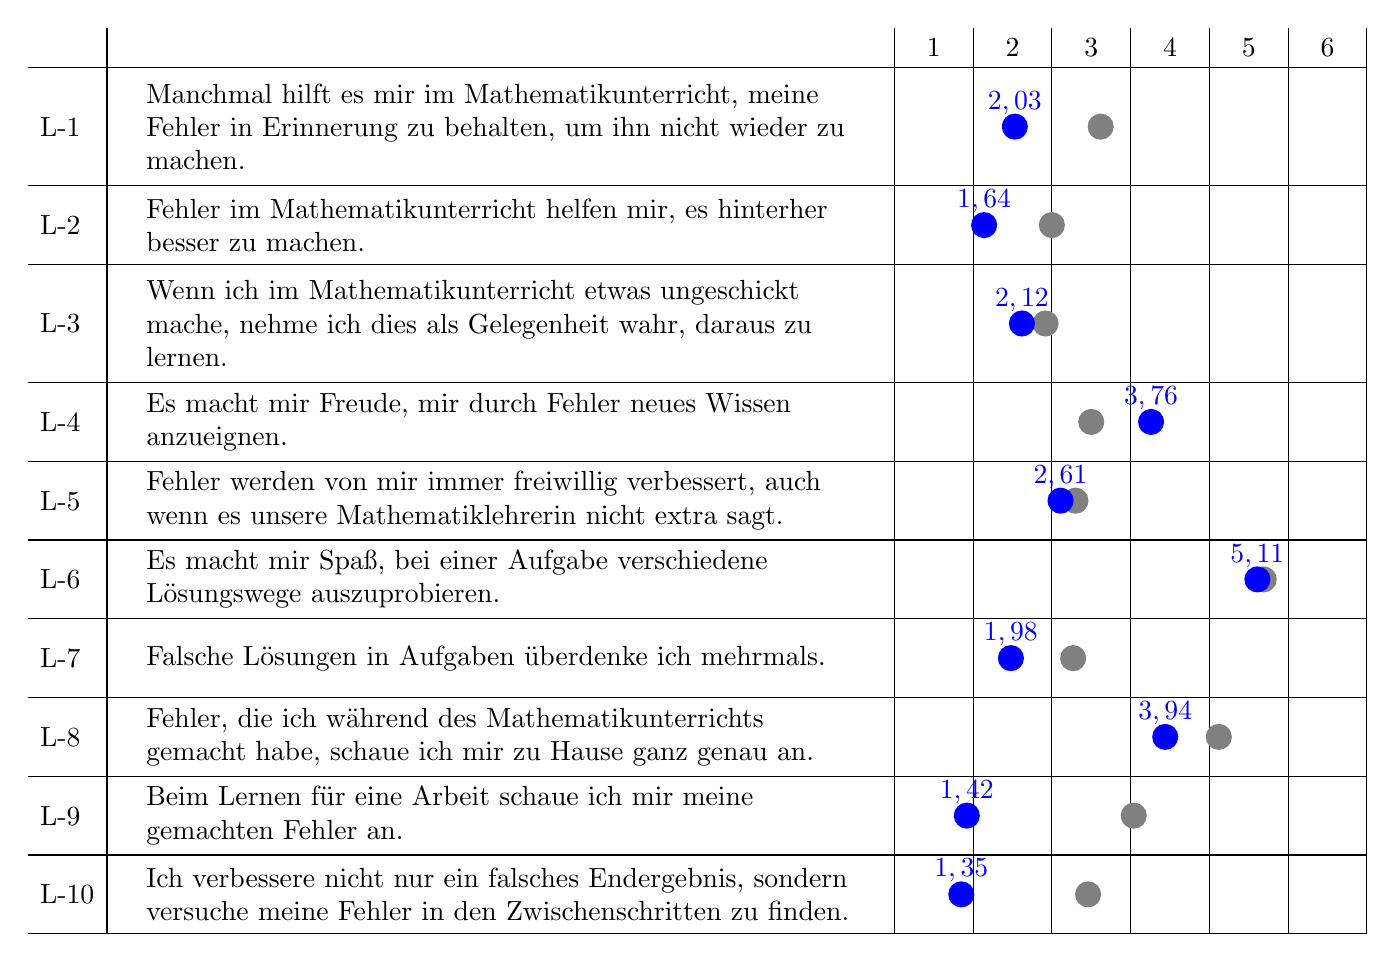
\begin{tikzpicture}

    \foreach \y in {0,1.5,2.5,4,5,6,7,8,9,10,11}
        \draw (-1, 0 - \y) -- (16, 0 - \y);
    \foreach \x in {0,10,11,12,13,14,15,16}
        \draw (0 + \x, 0.5) -- (0 + \x, - 11);
    
    \node at (10.5, 0.25) {$1$};
    \node at (11.5, 0.25) {$2$};
    \node at (12.5, 0.25) {$3$};
    \node at (13.5, 0.25) {$4$};
    \node at (14.5, 0.25) {$5$};
    \node at (15.5, 0.25) {$6$};

    \node[thick, circle, fill=gray, minimum width=0.25] (1) at (9.5 + 3.12, -0.75) {};
    \node[thick, align=left, text width=1cm] at (-0.35, -0.75) {L-1};
    \node[thick, align=left, text width=9cm] at (5, -0.75) {Manchmal hilft es mir im Mathematikunterricht, meine Fehler in Erinnerung zu behalten, um ihn nicht wieder zu machen.};
    \node[thick, circle, fill=blue, minimum width=0.25] (1) at (9.5 + 2.03, -0.75) {};
    \node[thick, blue] at (9.5 + 2.03, -0.45) {$2,03$};

    \node[thick, circle, fill=gray, minimum width=0.25] (2) at (9.5 + 2.5, -2) {};
    \node[thick, align=left, text width=1cm] at (-0.35, -2) {L-2};
    \node[thick, align=left, text width=9cm] at (5, -2) {Fehler im Mathematikunterricht helfen mir, es hinterher besser zu machen.};
    \node[thick, circle, fill=blue, minimum width=0.25] (2) at (9.5 + 1.64, -2) {};
    \node[thick, blue] at (9.5 + 1.64, -1.7) {$1,64$};

    \node[thick, circle, fill=gray, minimum width=0.25] (3) at (9.5 + 2.42, -3.25) {};
    \node[thick, align=left, text width=1cm] at (-0.35, -3.25) {L-3};
    \node[thick, align=left, text width=9cm] at (5, -3.25) {Wenn ich im Mathematikunterricht etwas ungeschickt mache, nehme ich dies als Gelegenheit wahr, daraus zu lernen.};
    \node[thick, circle, fill=blue, minimum width=0.25] (3) at (9.5 + 2.12, -3.25) {};
    \node[thick, blue] at (9.5 + 2.12, -2.95) {$2,12$};

    \node[thick, circle, fill=gray, minimum width=0.25] (4) at (9.5 + 3, -4.5) {};
    \node[thick, align=left, text width=1cm] at (-0.35, -4.5) {L-4};
    \node[thick, align=left, text width=9cm] at (5, -4.5) {Es macht mir Freude, mir durch Fehler neues Wissen anzueignen.};
    \node[thick, circle, fill=blue, minimum width=0.25] (4) at (9.5 + 3.76, -4.5) {};
    \node[thick, blue] at (9.5 + 3.76, -4.2) {$3,76$};

    \node[thick, circle, fill=gray, minimum width=0.25] (5) at (9.5 + 2.8, -5.5) {};
    \node[thick, align=left, text width=1cm] at (-0.35, -5.5) {L-5};
    \node[thick, align=left, text width=9cm] at (5, -5.5) {Fehler werden von mir immer freiwillig verbessert, auch wenn es unsere Mathematiklehrerin nicht extra sagt.};
    \node[thick, circle, fill=blue, minimum width=0.25] (5) at (9.5 + 2.61, -5.5) {};
    \node[thick, blue] at (9.5 + 2.61, -5.2) {$2,61$};

    \node[thick, circle, fill=gray, minimum width=0.25] (6) at (9.5 + 5.19, -6.5) {};
    \node[thick, align=left, text width=1cm] at (-0.35, -6.5) {L-6};
    \node[thick, align=left, text width=9cm] at (5, -6.5) {Es macht mir Spaß, bei einer Aufgabe verschiedene Lösungswege auszuprobieren.};
    \node[thick, circle, fill=blue, minimum width=0.25] (6) at (9.5 + 5.11, -6.5) {};
    \node[thick, blue] at (9.5 + 5.11, -6.2) {$5,11$};

    \node[thick, circle, fill=gray, minimum width=0.25] (7) at (9.5 + 2.77, -7.5) {};
    \node[thick, align=left, text width=1cm] at (-0.35, -7.5) {L-7};
    \node[thick, align=left, text width=9cm] at (5, -7.5) {Falsche Lösungen in Aufgaben überdenke ich mehrmals.};
    \node[thick, circle, fill=blue, minimum width=0.25] (7) at (9.5 + 1.98, -7.5) {};
    \node[thick, blue] at (9.5 + 1.98, -7.2) {$1,98$};

    \node[thick, circle, fill=gray, minimum width=0.25] (7) at (9.5 + 4.62, -8.5) {};
    \node[thick, align=left, text width=1cm] at (-0.35, -8.5) {L-8};
    \node[thick, align=left, text width=9cm] at (5, -8.5) {Fehler, die ich während des Mathematikunterrichts gemacht habe, schaue ich mir zu Hause ganz genau an.};
    \node[thick, circle, fill=blue, minimum width=0.25] (7) at (9.5 + 3.94, -8.5) {};
    \node[thick, blue] at (9.5 + 3.94, -8.2) {$3,94$};

    \node[thick, circle, fill=gray, minimum width=0.25] (7) at (9.5 + 3.54, -9.5) {};
    \node[thick, align=left, text width=1cm] at (-0.35, -9.5) {L-9};
    \node[thick, align=left, text width=9cm] at (5, -9.5) {Beim Lernen für eine Arbeit schaue ich mir meine gemachten Fehler an.};
    \node[thick, circle, fill=blue, minimum width=0.25] (7) at (9.5 + 1.42, -9.5) {};
    \node[thick, blue] at (9.5 + 1.42, -9.2) {$1,42$};

    \node[thick, circle, fill=gray, minimum width=0.25] (7) at (9.5 + 2.96, -10.5) {};
    \node[thick, align=left, text width=1cm] at (-0.35, -10.5) {L-10};
    \node[thick, align=left, text width=9cm] at (5, -10.5) {Ich verbessere nicht nur ein falsches Endergebnis, sondern versuche meine Fehler in den Zwischenschritten zu finden.};
    \node[thick, circle, fill=blue, minimum width=0.25] (7) at (9.5 + 1.35, -10.5) {};
    \node[thick, blue] at (9.5 + 1.35, -10.2) {$1,35$};

    %\draw[color=blue, thick] (1) to (2) to (3) to (4) to (5);

  \end{tikzpicture}%
\end{document}
